\documentclass{cours}

\title{\textsc{Etude Computationnelle de la Stabilité Interlangue des Catégories Morphosyntaxiques}\\
{\small Rapport de Stage de L3} }
\author{Matthieu Boyer}

\newcommand{\codedir}{Morphosyntactic-Categories_Code}
\usepackage{nicematrix}

\begin{document}

    \begin{abstract}
        Dans ce rapport, nous nous intéressons à la stabilité interlangue des catégories morphosyntaxiques.
        Nous avons quantifié la manière dont différentes catégories descriptives d'un langage ont différentes
        significations dans différents langages,
        et particulièrement la manière dont un concept est matérialisé dans différents langages.
    \end{abstract}


    \section{Pourquoi?}\label{sec:Pourquoi?}
    Cette citation de Martin Haspelmath sur la différence entre une catégorie linguistique descriptive dans un langage et une catégorie linguistique comparative dans le méta-langage est le point de départ de notre étude.
    \begin{quote}
        There is a fundamental distinction between language-particular categories of languages (which descriptive
        linguists must describe by descriptive categories of their descriptions) and comparative concepts (which
        comparative linguists may use to compare languages).
    \end{quote}
    {\flushright
    {\textit{Martin Haspelmath}, \textsc{How comparative concepts and descriptive linguistic categories are different}}}
    Selon Haspelmath, il est possible que la manière de décrire les langues en linguistique soit basée sur des envies de comparaison, parfois mal placées.
    Dans ce rapport, nous allons donc nous intéresser à la notion fondamentale de catégorie morphosyntaxique, et
    comparer les descriptions dans différents langages de catégories linguistiques comparatives.\\
    Pour ce faire, nous allons considérer que les relations de dépendances (\textit{reldep}
    ) décrites par les annotations de \textsc{Universal Dependencies} (UD)
    sont une manière de représenter des catégories comparatives.


    \section{Première Approche.}\label{sec:premiere-approche.}
    Nous considérons tout d'abord que chaque \textit{reldep} décrit une unique catégorie comparative et que plusieurs \textit{reldep} ne peuvent instancier une même catégorie comparative.
    En comptant le nombre d'instances de chaque \textit{reldep} pour un mot vérifiant une propriété grammaticale de la langue (i.e.\ une catégorie descriptive, que l'on représente par une \textit{feature} d'UD, typiquement les cas pour des langues en utilisant), on obtient une représentation vectorielle des catégories descriptives et on peut donc mesurer la proximité de deux catégories descriptives dans deux langues différentes.
    Les corpus utilisés dans cette première partie sont ceux du projet \textsc{Universal Dependencies}, accessibles en ligne.

    \subsection{Avec la distance Cosinus}
    On mesure en utilisant la distance Cosinus entre deux vecteurs\footnote{$d_{\cos}(v_{1},v_{2}) = \frac{\scalar{v_{1}\mid v_{2}}}{\norm{v_{1}}\norm{v_{2}}}$}, la proximité entre ceux ci. On obtient alors les résultats suivants pour quelques cas:


    \renewcommand{\arraystretch}{1.1}
\begin{table}[H]
	\centering
	\resizebox{\textwidth}{!}{\begin{NiceTabular}{ccccccccc}
		Proximity with: & Abl & Acc & Dat & Gen & Ins & Loc & Nom & Voc \\
		First Quartile & 0.028 & 0.394 & 0.030 & 0.020 & 0.042 & 0.014 & 0.038 & 0.000 \\
		Median & 0.202 & 0.711 & 0.181 & 0.123 & 0.236 & 0.176 & 0.137 & 0.007 \\
		Third Quartile & 0.393 & 0.860 & 0.379 & 0.302 & 0.408 & 0.381 & 0.272 & 0.040 \\
		Mean & 0.242 & 0.616 & 0.236 & 0.196 & 0.255 & 0.230 & 0.188 & 0.042 \\
	\CodeAfter
		\begin{tikzpicture}
			\foreach \i in {1,...,6}
				{\draw[draw=vulm] (1|-\i) -- (10|-\i);}
			\draw[draw=vulm] (2|-1)--(2|-6);\end{tikzpicture}
	\end{NiceTabular}}
	\caption{Proximities for Case=Acc}
\end{table}

    \renewcommand{\arraystretch}{1.1}
\begin{table}[H]
	\centering
	\begin{NiceTabular}{cccccccc}
		Proximity with: & Case=Nom & Case=Acc & Case=Dat & Case=Gen & Case=Voc & Case=Loc & Case=Abl \\
		Median & 0.0 & 0.0 & 0.0 & 0.0 & 0.0 & 0.0 & 0.0 \\
		Mean & 0.03328 & 0.05376 & 0.09264 & 0.05258 & 0.00444 & 0.05714 & 0.0343 \\
		NLow & 57901 & 38008 & 28140 & 34565 & 21502 & 16842 & 8188 \\
		NHigh & 412 & 2446 & 9658 & 2324 & 12 & 7240 & 4837 \\
		First Quartile & 0.0 & 0.0 & 0.0 & 0.0 & 0.0 & 0.0 & 0.0 \\
		Third Quartile & 0.0 & 0.0 & 0.0 & 0.0 & 0.0 & 0.0 & 0.0 \\
	\CodeAfter
		\begin{tikzpicture}
			\foreach \i in {1,...,8}
				{\draw[draw=vulm] (1|-\i) -- (9|-\i);}
			\draw[draw=vulm] (2|-1)--(2|-8);\end{tikzpicture}
	\end{NiceTabular}
	\caption{Proximities for Case=Dat}
\end{table}

    \renewcommand{\arraystretch}{1.1}
\begin{table}[H]
	\centering
	\resizebox{\textwidth}{!}{\begin{NiceTabular}{ccccccccc}
		Proximity with: & Abl & Acc & Dat & Gen & Ins & Loc & Nom & Voc \\
		First Quartile & 0.037 & 0.020 & 0.022 & 0.032 & 0.056 & 0.027 & 0.026 & 0.000 \\
		Median & 0.198 & 0.123 & 0.134 & 0.317 & 0.249 & 0.188 & 0.104 & 0.006 \\
		Third Quartile & 0.416 & 0.302 & 0.341 & 0.823 & 0.449 & 0.400 & 0.225 & 0.047 \\
		Mean & 0.259 & 0.196 & 0.214 & 0.421 & 0.282 & 0.243 & 0.159 & 0.058 \\
	\CodeAfter
		\begin{tikzpicture}
			\foreach \i in {1,...,6}
				{\draw[draw=vulm] (1|-\i) -- (10|-\i);}
			\draw[draw=vulm] (2|-1)--(2|-6);\end{tikzpicture}
	\end{NiceTabular}}
	\caption{Proximities for Case=Gen}
\end{table}

    \begin{table}[H]
	\centering
	\begin{NiceTabular}{ccccccc}
		Proximity with: & Case=Nom & Case=Acc & Case=Dat & Case=Gen & Case=Voc & Case=Loc \\
		Median & 0.44588 & 0.46849 & 0.48794 & 0.46892 & 0.51927 & 0.57887 \\
		Mean & 0.49841 & 0.51443 & 0.51995 & 0.50402 & 0.54114 & 0.58953 \\
		NLow & 27886 & 21110 & 21518 & 21266 & 11000 & 18048 \\
		NHigh & 29971 & 27910 & 28499 & 25073 & 16744 & 45864 \\
		First Quartile & 0.23495 & 0.26545 & 0.27671 & 0.26711 & 0.26242 & 0.3383 \\
		Third Quartile & 0.77133 & 0.76979 & 0.7566 & 0.72731 & 0.83677 & 0.87388 \\
	\CodeAfter
		\begin{tikzpicture}
			\foreach \i in {1,...,8}
				{\draw[draw=vulm] (1|-\i) -- (8|-\i);}
			\draw[draw=vulm] (2|-1)--(2|-8);\end{tikzpicture}
	\end{NiceTabular}
	\caption{Proximities for Case=Loc}
\end{table}

    \renewcommand{\arraystretch}{1.1}
\begin{table}[H]
	\centering
	\begin{NiceTabular}{cccccccc}
		Proximity with: & Case=Nom & Case=Acc & Case=Dat & Case=Gen & Case=Voc & Case=Loc & Case=Abl \\
		Median & 0.0 & 0.0 & 0.0 & 0.0 & 0.0 & 0.0 & 0.0 \\
		Mean & 0.26295 & 0.07799 & 0.04112 & 0.06237 & 0.01181 & 0.02566 & 0.0162 \\
		NLow & 18404 & 80944 & 75574 & 79415 & 35362 & 48157 & 28185 \\
		NHigh & 54192 & 2105 & 506 & 2145 & 254 & 211 & 107 \\
		First Quartile & 0.0 & 0.0 & 0.0 & 0.0 & 0.0 & 0.0 & 0.0 \\
		Third Quartile & 0.54978 & 0.0799 & 0.01559 & 0.05144 & 0.0 & 0.0 & 0.0 \\
	\CodeAfter
		\begin{tikzpicture}
			\foreach \i in {1,...,8}
				{\draw[draw=vulm] (1|-\i) -- (9|-\i);}
			\draw[draw=vulm] (2|-1)--(2|-8);\end{tikzpicture}
	\end{NiceTabular}
	\caption{Proximities for Case=Nom}
\end{table}

    \begin{table}[H]
	\centering
	\begin{NiceTabular}{ccccccc}
		Proximity with: & Case=Nom & Case=Acc & Case=Dat & Case=Gen & Case=Voc & Case=Loc \\
		Median & 0.53652 & 0.52529 & 0.49388 & 0.55171 & 0.88359 & 0.56814 \\
		Mean & 0.55947 & 0.54856 & 0.53176 & 0.55858 & 0.76794 & 0.57436 \\
		NLow & 10168 & 9358 & 10354 & 8638 & 2688 & 6416 \\
		NHigh & 18219 & 14842 & 13198 & 14931 & 33512 & 12001 \\
		First Quartile & 0.27545 & 0.27187 & 0.24879 & 0.28231 & 0.63158 & 0.27575 \\
		Third Quartile & 0.87261 & 0.83938 & 0.81784 & 0.84647 & 0.97788 & 0.8884 \\
	\CodeAfter
		\begin{tikzpicture}
			\foreach \i in {1,...,8}
				{\draw[draw=vulm] (1|-\i) -- (8|-\i);}
			\draw[draw=vulm] (2|-1)--(2|-8);\end{tikzpicture}
	\end{NiceTabular}
	\caption{Proximities for Case=Voc}
\end{table}

    \renewcommand{\arraystretch}{1.1}
\begin{table}[H]
	\centering
	\begin{NiceTabular}{cccccccc}
		Proximity with: & Case=Nom & Case=Acc & Case=Dat & Case=Gen & Case=Voc & Case=Loc & Case=Abl \\
		Median & 0.0 & 0.0 & 0.0 & 0.0 & 0.0 & 0.0 & 0.0 \\
		Mean & 0.00599 & 0.00569 & 0.0167 & 0.0087 & 0.00033 & 0.01607 & 0.02558 \\
		NLow & 7840 & 6501 & 3013 & 6616 & 1545 & 2368 & 2056 \\
		NHigh & 49 & 453 & 2916 & 457 & 0 & 3704 & 6022 \\
		First Quartile & 0.0 & 0.0 & 0.0 & 0.0 & 0.0 & 0.0 & 0.0 \\
		Third Quartile & 0.0 & 0.0 & 0.0 & 0.0 & 0.0 & 0.0 & 0.0 \\
	\CodeAfter
		\begin{tikzpicture}
			\foreach \i in {1,...,8}
				{\draw[draw=vulm] (1|-\i) -- (9|-\i);}
			\draw[draw=vulm] (2|-1)--(2|-8);\end{tikzpicture}
	\end{NiceTabular}
	\caption{Proximities for Case=Abl}
\end{table}

    Toutefois, cette méthode est très limitée. En effet, on ne considère ici que 9 des 45 cas définis dans au moins un corpus. Par ailleurs, les résultats donnés ici sont à pondérer par la présence de nombreux corpus/langages ne possédant pas au moins l'un des cas ci-dessus, ce qui amène à une représentation trop brouillée des informations.

    \subsection{Avec l'algorithme de \textsc{Zassenhaus}}
    On considère les espaces vectoriels engendrés par la représentation vectorielle du système de cas d'une langue, que l'on appellera \textit{espaces de cas}.
    Ceux-ci sont d'une certaine dimension finie.
    On applique alors sur toute paire de système de cas l'algorithme de Zassenhaus, permettant de générer une base de l'espace somme et de l'espace intersection.
    Toutefois, la grande variance au niveau des coordonnées, et la trop faible dimension (au plus 45, mais souvent de l'odrdre de 5) dans un grand espace (dimension 228), rend l'intersection toujours nulle numériquement.
    Par ailleurs, cet algorithme est très lent à exécuter car il demande de nombreux appels mémoire pour obtenir la matrice de l'espace de cas de chaque paire de cas, et demande de trouver une base de l'espace de colonne, ce qui est non-trivialement la matrice.

    \subsection{Angle entre Cas et Système de Cas}
    On considère à nouveau la distance cosinus, mais cette fois-ci, non pas entre deux vecteurs, mais entre un vecteur et un espace de cas.
    Ceci est fait en considérant le projeté orthogonal d'un vecteur sur un espace de cas et en mesurant l'angle entre les deux (ou la distance cosinus).
    En observant les données de plus près, on trouve une anomalie: l'angle entre le vocatif du farsi et le système de cas arabe est de l'ordre de $10^{-16}$.
    En regardant de plus près les corpus farsis\footnote{et non pas les dindes.}, on observe que cela découle d'une idiosyncracie dans les annotations.
    En farsi, le lemme (unité morphologique abstraite: \textsl{fais} et \textsl{fait} sont deux graphies du même lemme \textsl{faire}, conjugué à deux personnes différentes)
    % \textit{ای}\footnote{Translit=āī}
    est décrit comme une interjection portant le vocatif et se reliant à un nom au cas absolu par la relation de transmission de cas (c'est à dire de marquer le cas pour un autre mot).
    Ce lemme agit donc en réalité plus comme une apposition.
    Le vocatif n'apparaît que très peu en farsi, et majoritairement dans cette situation.
    Ainsi, il semble que nous ne pouvons pas tirer d'enseignements du farsi vers une autre langue, du moins sur le système de cas.
    Il semble toutefois bon de noter qu'il y a sans doute de nombreuses autres anomalies du style dans les corpus.

    Par ailleurs, il n'est pas rare qu'au sein d'une même langue, deux corpus produisent des résultats assez différents. Ceci peut venir de la variance des phrases considérées, mais plus souvent de la présence ou non des reldeps \texttt{conj, case} et de la manière d'annoter le cas d'une apposition (cf. supra).

    \subsection{Distance Euclidienne}
    On considère cette fois la distance euclidienne entre tous deux vecteurs, qu'on aura au préalable normalisés pour qu'ils représentent des distributions de probabilité.
    On utilise ces données pour déterminer, entre deux corpus (ici le Czech-CLTT et le Russian-GSD), quel cas de l'autre langage est le plus proche d'un cas du premier.
    On obtient qu'ici, le datif russe est plus proche du génitif tchèque que du datif tchèque.
    \begin{table}[H]
	    \centering
    \begin{tabular}{>{\tt}r|cccc}
        \toprule
        &Dat RU & Gen CZ & Gen RU & Dat CZ\\
        \midrule
        Total & 1711 & 2631 & 2070 & 277\\
        obl & 450 & 208 & 219 & 48\\
        iobj & 340 & 0 & 0 & 0\\
        amod & 243 & 736 & 475 & 54\\
        nmod & 300 & 1000 & 980 & 24\\
        conj & 112 & 225 & 84 & 21\\
        case & 0 & 340 & 1 & 87\\
        det & 34 & 80 & 79 & 3\\
        \bottomrule
    \end{tabular}
	\caption{Extraits des Vecteurs de Reldep pour le Russe et le Tchèque}
    \end{table}

    En considérant le graphe orienté des plus proches voisins, on remarque que celui-ci ne peut pas avoir de $n$-cycle pour $n \geq 3$ et décrit des relations de proximité minimale.
    On obtient alors le graphe suivant pour le tchèque et le russe:
    \begin{figure}[H]
	    \centering
	    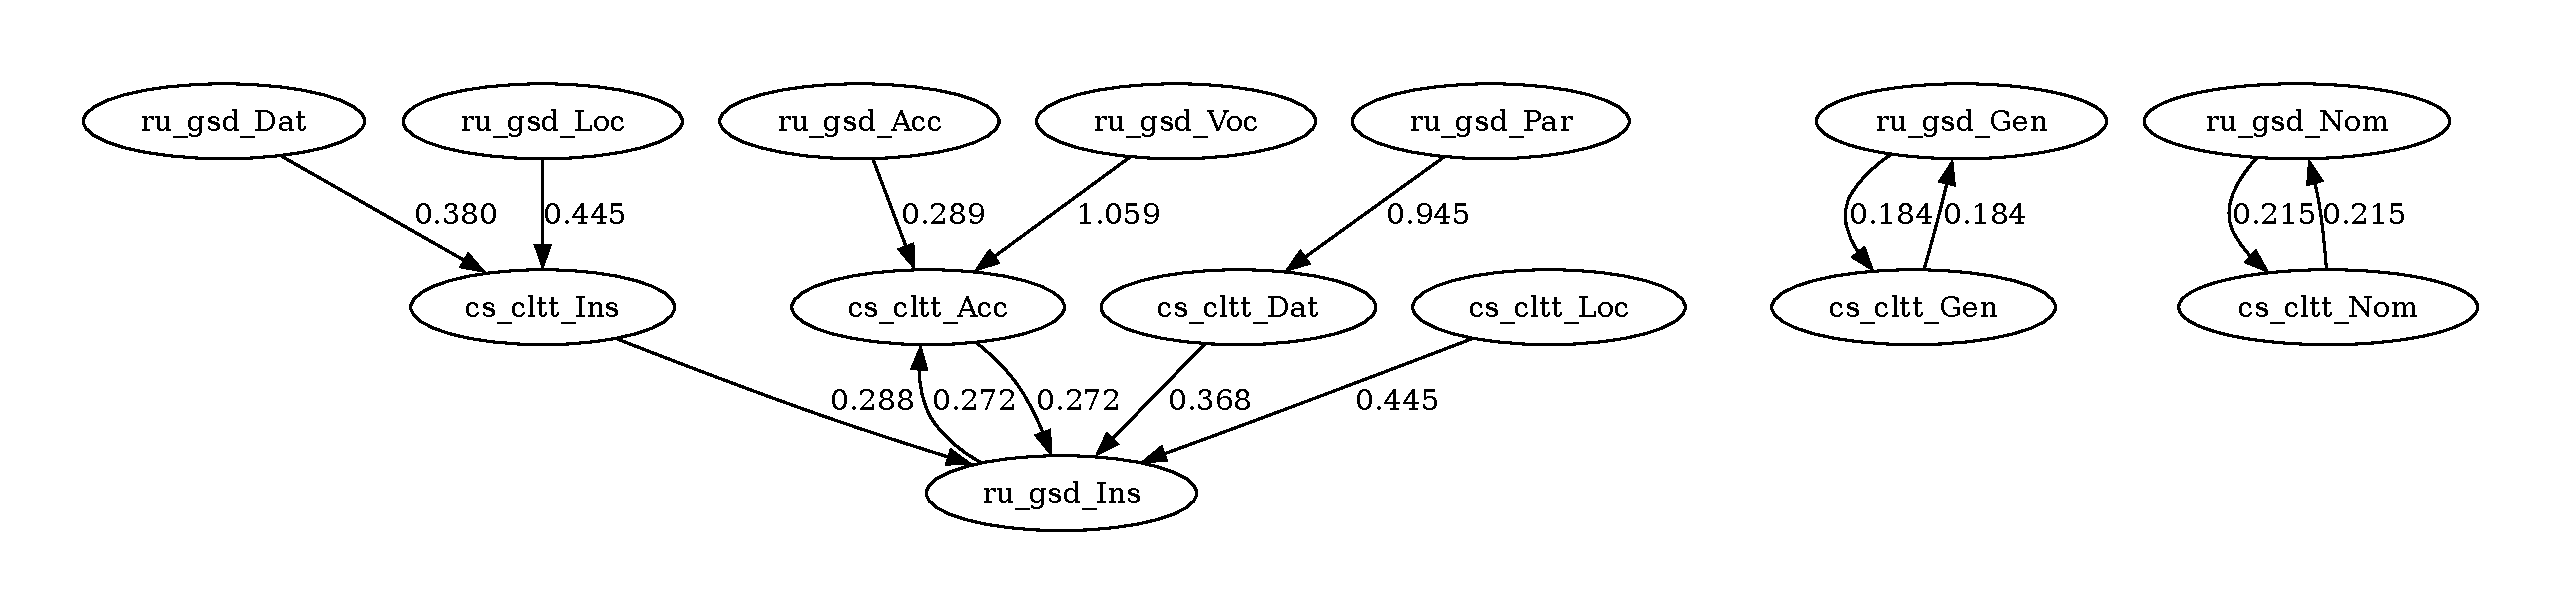
\includegraphics[width=\textwidth]{\codedir/Figures/gnn_ru_gsd_cs_cltt.pdf}
    \end{figure}
    \begin{figure}[H]
	    \centering
	    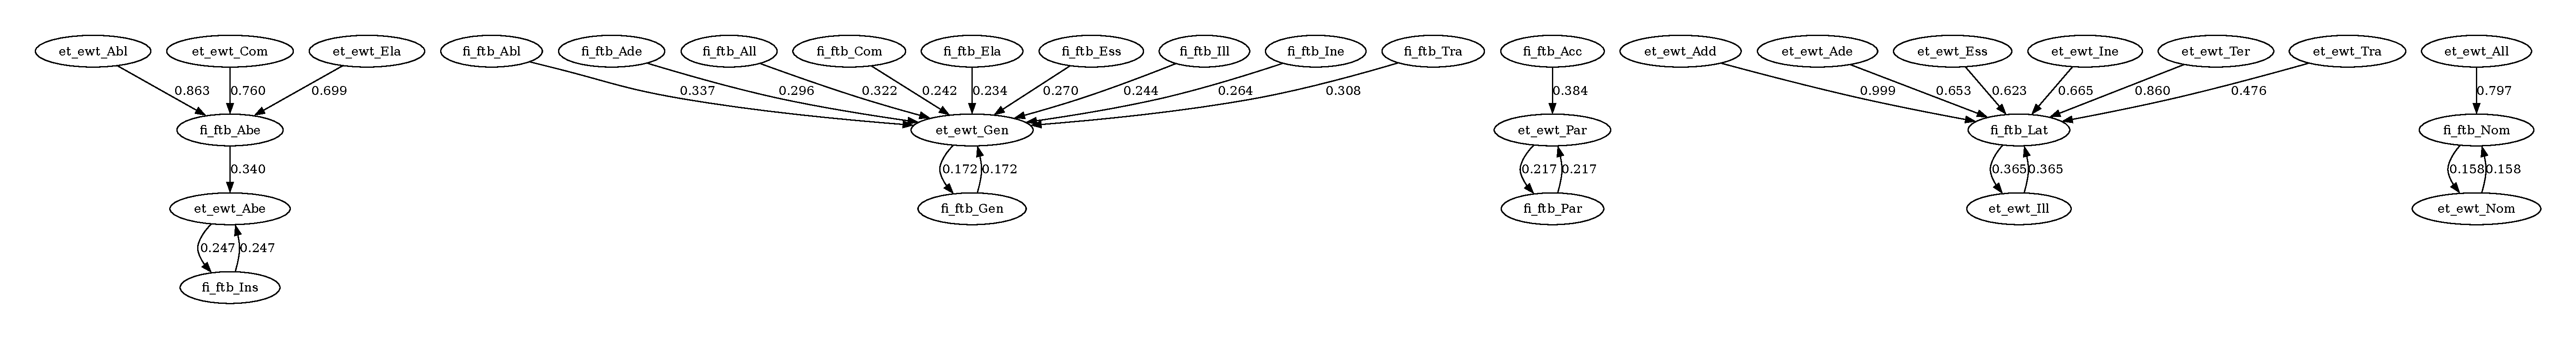
\includegraphics[width=\textwidth]{\codedir/Figures/gnn_fi_ftb_et_ewt.pdf}
    \end{figure}
    On enlève ensuite \texttt{conj, det} puisque ces reldep démontrent l'accord vers la tête, et donc des doublons dans les données et on se restreint aux mots de nature \textit{Nom}. Ceci permet d'éviter la variance liée aux adjectifs, pronoms et dans de rares cas (ceux-ci restant majoritairement au cas absolu) aux adverbes.
    On enlève aussi case, qui souvent (notamment visible dans l'exemple ci-dessous), est utilisé pour marquer le cas avec une apposition (sur, sous), et ceci dépend très fortement de la personne qui a annoté le corpus, et de l'usage dans les grammaires du langage.\\
    On obtient alors le graphe suivant pour le tchèque et le russe:
    \begin{figure}[H]
	    \centering
	    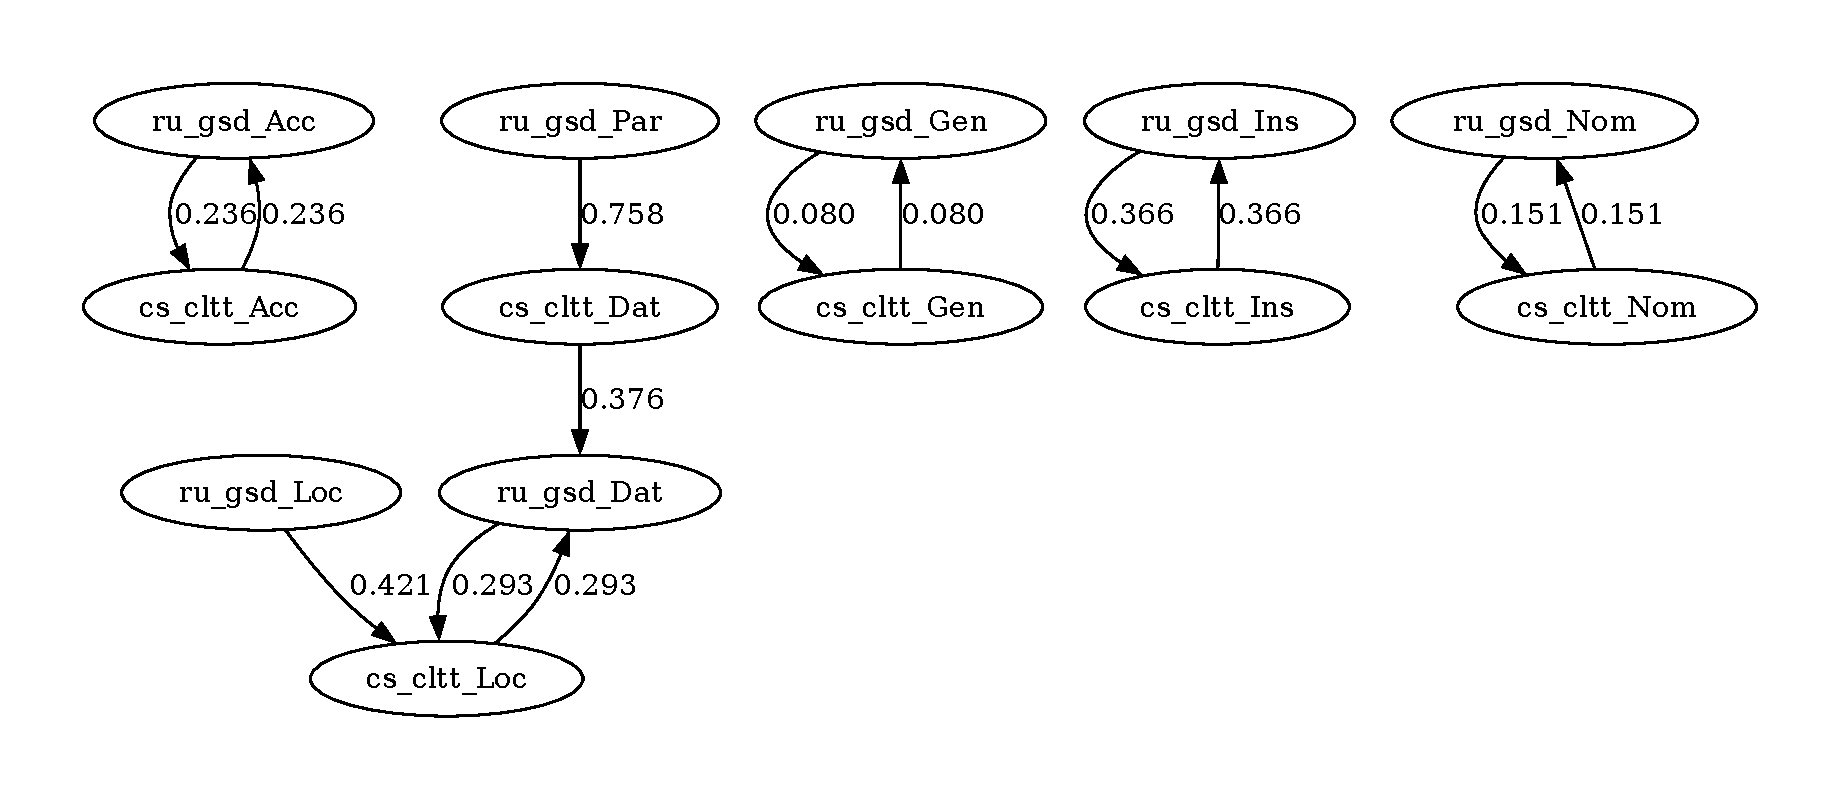
\includegraphics[width=\textwidth]{\codedir/Figures/gnn_ru_gsd_cs_cltt_Nouns_Only.pdf}
    \end{figure}
    \begin{figure}[H]
	    \centering
	    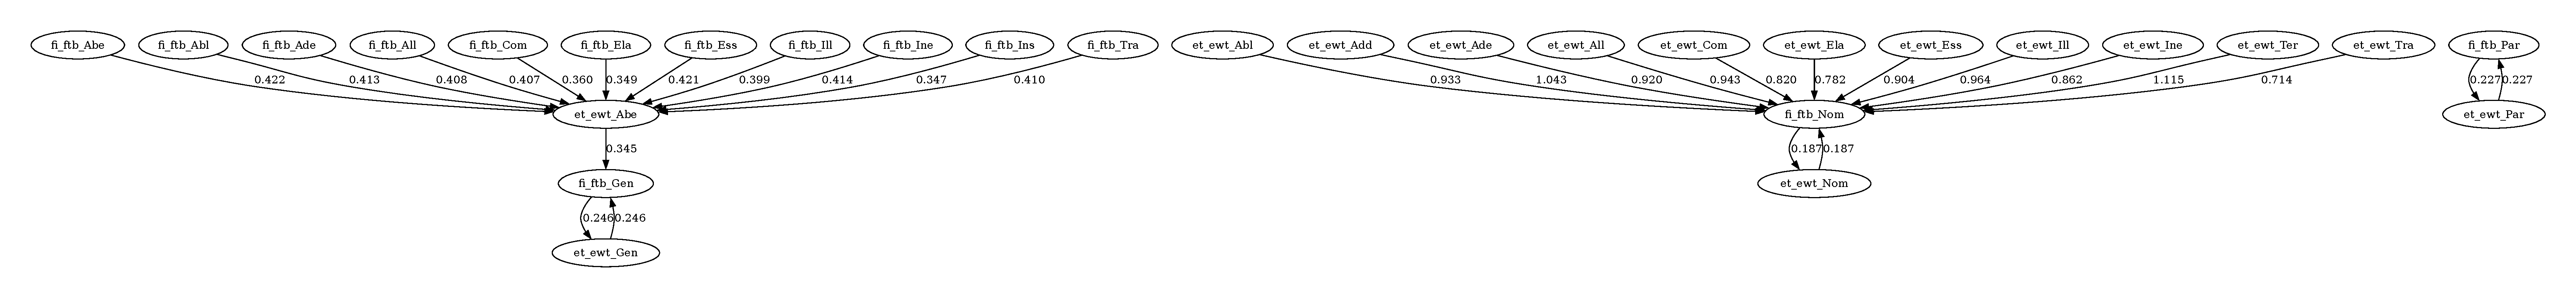
\includegraphics[width=\textwidth]{\codedir/Figures/gnn_fi_ftb_et_ewt_Nouns_Only.pdf}
    \end{figure}



\end{document}
